\documentclass[a4paper,12pt,oneside]{report}
\usepackage[spanish,USenglish]{babel} % espanol, ingles
\usepackage{amsmath,amssymb}
\usepackage{listings}
\usepackage{latexsym}
\usepackage{pdfpages}
\usepackage[normalem]{ulem}
\usepackage{graphicx}
\usepackage{graphics}
\usepackage{qtree}
\usepackage{url}
\usepackage{array}
\usepackage{float}
\usepackage[top=1in,bottom=1in,left=1.25in,right=1.25in]{geometry}
\bibliographystyle{ieeetr}
\title{Bases de Datos Temporales, Espaciales y Espacio-Temporales}
\date{\today}
\author{Nicol\'as Del Piano}
\date{}
\newcommand{\mychapter}[2]{
    \setcounter{chapter}{#1}
    \setcounter{section}{0}
    \chapter*{#2}
    \addcontentsline{toc}{chapter}{#2}
}
\begin{document}
\selectlanguage{spanish}
\maketitle
\tableofcontents
\newpage

\mychapter{0}{Res\'umen}
Este trabajo presenta una introducci\'on hacia las Bases de Datos Temporales, Espaciales y Espacio-Temporales. Las Bases de Datos Temporales (\textit{Temporal Databases}) est\'an dise\~nadas para la captura de informaci\'on que var\'ia en el tiempo. Las Bases de Datos Espaciales (\textit{Spatial Databases}) fueron concebidas por la necesidad de registrar el cambio geogr\'afico y f\'isico de cierta informaci\'on. Por \'ultimo, las Bases de Datos Espacio-Temporales (\textit{Spatio-Temporal Databases}) son el resultado de la uni\'on de las capacidades y propiedades ofrecidas por ambos tipos de Bases de Datos. Primero se presentar\'an conceptos de Bases de Datos cl\'asicas, para luego abordar m\'as claramente los temas centrales de esta monograf\'ia. El segundo cap\'itulo presenta de una manera detallada las Bases de Datos Temporales, el tercero lo hace para las Espaciales, y el cuarto para las Espacio-Temporales. Por \'ultimo se abordan t\'opicos generales relacionados con estos tipos de Bases de Datos.
\mychapter{1}{Introducci\'on}
Hoy en d\'ia, la cantidad de informaci\'on que manejan las corporaciones y empresas es gigantesca. Por esta raz\'on, es necesario el uso de una herramienta que provea una forma de gestionar adecuadamente esta informaci\'on. Este es el prop\'osito de las Bases de Datos: brindar al usuario una forma de controlar el acceso, almacenamiento y administraci\'on de los datos de la entidad en cuesti\'on.\\
Con la aparici\'on de nuevas tecnolog\'ias, el surgimiento de nuevas necesidades fue inevitable, implicando que las Bases de Datos Relacionales no sean una bala de plata (aunque sean las m\'as usadas actualmente) para resolver todos los problemas de gesti\'on de datos. Surgieron conceptos como Miner\'ia de Datos, Data Warehouse y Big Data: la informaci\'on ya no tiene la misma dimensi\'on que antes. Fue entonces cuando el Modelo Relacional cl\'asico necesitaba extenderse para representar eficientemente datos que var\'ien en tiempo y espacio.\\
Las Bases de Datos Temporales se encargan del dominio del tiempo y su relaci\'on con los datos, permite analizar la historia y controlar la validez temporal de los mismos. Una gran variedad de aplicaciones del mundo real manejan datos variables en el tiempo: control de inventario, registros m\'edicos, operaciones bancarias, sistemas de informaci\'on geogr\'afica, gesti\'on de reservas, aplicaciones cient\'ificas, etc\'etera. Esta necesidad de referencias temporales justifica la creaci\'on de un modelo de datos temporal.\\
Las Bases de Datos Espaciales extienden el modelo para representar el dominio espacial, con estructuras que puedan identificar un objeto en el espacio. Deben permitir la descripci\'on de objetos espaciales mediante tres caracter\'isticas: atributos, localizaci\'on y topolog\'ia. Adem\'as deben proveer tipos de datos espaciales para estructurar entidades geom\'etricas en el espacio. Existen diversas \'areas donde la gesti\'on de informaci\'on geom\'etrica, geogr\'afica o espacial es crucial: Sistemas de Informaci\'on Geogr\'afica, Bases de Datos multimedia, im\'agenes satelitales, ciencias ambientales, astronom\'ia.\\
El objetivo de las Bases de Datos Espacio-Temporales es extender los modelos de informaci\'on espacial para inclu\'ir el tiempo y describir en forma m\'as din\'amica la realidad que se quiere representar. El modelo espacio-temporal abarca aplicaciones demogr\'aficas, ecol\'ogicas, relacionadas con marketing, militares, urban\'isticas y de fen\'omenos naturales, entre otras.\\
\mychapter{2}{Bases de Datos Relacionales}
\mychapter{3}{Bases de Datos Temporales}
El tiempo es un aspecto importante para los fen\'omenos del mundo real: los eventos ocurren en momentos de tiempo espec\'ificos.\\
A veces nos interesa saber con cierta certeza cu\'ando ocurri\'o tal evento, y poder compararlo con otros para obtener informaci\'on de inter\'es.\\
Muchas de las \'areas donde se aplican las Bases de Datos tienen naturaleza temporal:
\begin{itemize}
\item Control de inventario.
\item Registros m\'edicos.
\item Sistemas de informaci\'on geogr\'afica.
\item Operaciones bancarias.
\item Data Warehousing.
\item Sistemas de control de reservas (aerol\'ineas, hoteles, etc).
\item Aplicaciones cient\'ificas.
\end{itemize}
\subsubsection*{Relaciones no temporales}
En la Figura 3.1 puede observarse una tabla relacional no temporal.
\begin{figure}[h]
\center
\includegraphics[scale=0.6]{temporal1.png}
\caption{Tabla relacional no temporal.}
\end{figure}
Cada tupla representa un hecho verdadero \textit{ahora}. Solo hay un estado representable de la Base de Datos: \textit{el actual} (\textit{current snapshot}).
A medida que el tiempo transcurre, los datos se van actualizando y modificando. Con este modelo, perdemos informaci\'on.\\
Las Bases de Datos convencionales representan el estado de la informaci\'on en un instante de tiempo dado. Aunque la Base de Datos es actualizada, estos cambios son vistos como modificaciones del estado actual y los datos obsoletos son borrados.\\
Por lo tanto, solo podemos utilizar la informaci\'on actual de la Base de Datos.\\
Esto genera un problema cuando queremos responder preguntas involucradas a intervalos de tiempo: \textit{?`Cu\'ales empleados percibieron un aumento el mes pasado?}
\subsubsection*{Bases de Datos Temporales: Definici\'on}
Un \textit{DBMS Temporal} es un Sistema de Gesti\'on de Bases de Datos que proporciona herramientas para el manejo y control de Bases de Datos Temporales.\\
Una \textit{Base de Datos Temporales} es una Base de Datos que tiene dimensi\'on del tiempo a trav\'es del almacenamiento de datos temporales.\\ Proporcionan un marco que mantiene la historia de los cambios que se produjeron en la fuente de datos. Est\'an dise\~nadas para la captura de la informaci\'on que var\'ia en el transcurso del tiempo (puede apreciarse esta relaci\'on en la Figura 3.2).
\begin{figure}[h]
\center \includegraphics[scale=0.4]{temporal2.jpg}
\caption{Relaci\'on tiempo y datos.}
\end{figure}
\subsubsection*{Datos Temporales}
Un \textit{Dato Temporal} es un dato convencional al que se le asocia un per\'iodo de tiempo para expresar valores temporales en la Base de Datos.\\
Este agregado de informaci\'on temporal se denomina \textit{time-stamping}. Al asociar el tiempo con la informaci\'on, es posible almacenar diferentes estados de una base de datos.
\subsubsection*{Dimensi\'on del Tiempo}
El tiempo es infinito, continuo y multidimensional \cite{snodgrass86}. Las computadoras no pueden representar informaci\'on continua, de hecho, se aproximan discretamente. As\'i, para representar una noci\'on del tiempo, se lo transforma en un conjunto discreto con una cierta granularidad. Por ejemplo, la sentencia \textit{Homero Simpson naci\'o el 12 de Mayo de 1956} tiene una granularidad de d\'ias.\\ 
Las Bases de Datos Temporales almacenan dos dimensiones de tiempo:
\begin{itemize}
\item Tiempo V\'alido
\item Tiempo Transaccional
\end{itemize}
El \textit{Tiempo V\'alido} representa cu\'ando un hecho tiene validez, es decir, es verdadero en el mundo real. El Tiempo V\'alido de un evento es el tiempo de un reloj en el que ese evento ocurri\'o \cite{snodgrass86}. Es independiente de si dicho evento fue registrado o no en la Base de Datos. Los Tiempos V\'alidos pueden encontrarse en el pasado, presente o futuro. Una de las caracter\'isticas es que todos los eventos tienen asociado un Tiempo V\'alido, pero no necesariamente son registrados. Adem\'as brindan la capacidad de gestionar la historia de la Base de Datos.\\
El \textit{Tiempo Transaccional} registra el per\'iodo de tiempo donde un hecho fue almacenado en la Base de Datos. Permiten realizar consultas que muestren el estado de la Base de Datos en un tiempo espec\'ifico. Este tiempo est\'a acotado en ambos extremos; la creaci\'on de la Base de Datos y el tiempo presente, es decir, los Datos Transaccionales viven solamente dentro de la vida de una Base de Datos. Una de las capacidades interesantes es que permiten volver hacia un estado anterior (\textit{roll-back}), ya que almacenan datos de las operaciones que se fueron haciendo.\\
Estas dos dimensiones son ortogonales. Un Modelo de Datos que no soporte ninguno de estas dimensiones se denomina \textit{snapshot}, ya que captura solamente una imagen de la Base de Datos. Si se brinda soporte para Tiempo V\'alido, entonces se cuenta con una Modelo de Datos \textit{hist\'orico}, mientras que uno que soporte Tiempo Transaccional solamente se denomina \textit{rollback}. En caso de que ambas dimensiones est\'en soportadas, se denomina \textit{bitemporal}.
\subsubsection*{Ejemplo}
An\'alizamos en forma no temporal y temporal el siguiente ejemplo:
\begin{itemize}
\item El Se\~nor X nace en Springfield el 12 de Mayo de 1956.
\begin{center}\includegraphics[width=1.8cm,height=2.3cm]{senorx.jpg}\end{center}
\item Su padre lo registra el 13 de Mayo de 1956.
\item Se muda a Arroyos Cipreses el 3 de Agosto de 1980, pero olvida registrarse; lo hace el 16 de Agosto del mismo a\~no.
\item Muere el 20 de Abril de 2004.
\end{itemize}
\subsubsection*{Ejemplo: no temporal}
\begin{center}
\begin{tabular}{|c|c|}
\hline
Nombre & ViveEn\\
\hline
Se\~nor X & Springfield\\
\hline
\end{tabular}
\\
\ \\
\begin{Huge}{$\Downarrow$}\end{Huge}\begin{small}{Update}\end{small}\\
\begin{tabular}{|c|c|}
\hline
Nombre & ViveEn\\
\hline
Se\~nor X & Arroyos Cipreses\\
\hline
\end{tabular}
\\
\ \\
\begin{Huge}{$\Downarrow$}\end{Huge}\begin{small}{Delete}\end{small}\\
\begin{tabular}{|c|c|}
\hline
Nombre & ViveEn\\
\hline
\sout{Se\~nor X} & \sout{Arroyos Cipreses}\\
\hline
\end{tabular}
\end{center}

\subsubsection*{Ejemplo: Tiempo V\'alido}
\begin{center}
\begin{tabular}{|c|c|c|c|}
\hline
Nombre & ViveEn & Valid-From & Valid-To\\
\hline
Se\~nor X & Springfield & 12-May-1956 & $\infty$\\
\hline
\end{tabular}
\\
\ \\
\begin{Huge}{$\Downarrow$}\end{Huge}\begin{small}{Update}\end{small}\\
\begin{tabular}{|c|c|c|c|}
\hline
Nombre & ViveEn & Valid-From & Valid-To\\
\hline
Se\~nor X & Springfield & 12-May-1956 & 2-Aug-1980\\
\hline
\end{tabular}
\\
\ \\
\begin{Huge}{$\Downarrow$}\end{Huge}\begin{small}{Insert}\end{small}\\
\begin{tabular}{|c|c|c|c|}
\hline
Nombre & ViveEn & Valid-From & Valid-To\\
\hline
Se\~nor X & Springfield & 12-May-1956 & 2-Aug-1980\\
\hline
Se\~nor X & Arroyos Cipreses & 3-Aug-1980 & $\infty$\\
\hline
\end{tabular}
\\
\ \\
\begin{Huge}{$\Downarrow$}\end{Huge}\begin{small}{Update}\end{small}\\
\begin{tabular}{|c|c|c|c|}
\hline
Nombre & ViveEn & Valid-From & Valid-To\\
\hline
Se\~nor X & Springfield & 12-May-1956 & 2-Aug-1980\\
\hline
Se\~nor X & Arroyos Cipreses & 3-Aug-1980 & 20-Apr-2004\\
\hline
\end{tabular}

\end{center}

\subsubsection*{Ejemplo: Tiempo Transaccional}
\begin{center}
\begin{tabular}{|c|c|c|c|}
\hline
Nombre & ViveEn & Transaction-From & Transaction-To\\
\hline
Se\~nor X & Springfield & 13-May-1956 & $\infty$\\
\hline
\end{tabular}
\\
\ \\
\begin{Huge}{$\Downarrow$}\end{Huge}\begin{small}{Insert}\end{small}\\
\begin{tabular}{|c|c|c|c|}
\hline
Nombre & ViveEn & Transaction-From & Transaction-To\\
\hline
Se\~nor X & Springfield & 13-May-1956 & 16-Aug-1980\\
\hline
Se\~nor X & Arroyos Cipreses & 16-Aug-1980 & $\infty$\\
\hline
\end{tabular}
\\
\ \\
\begin{Huge}{$\Downarrow$}\end{Huge}\begin{small}{Update}\end{small}\\
\begin{tabular}{|c|c|c|c|}
\hline
Nombre & ViveEn & Transaction-From & Transaction-To\\
\hline
Se\~nor X & Springfield & 13-May-1956 & 16-Aug-1980\\
\hline
Se\~nor X & Arroyos Cipreses & 16-Aug-1980 & 20-Apr-2004\\
\hline
\end{tabular}

\end{center}



\subsubsection*{Base de Datos Bitemporal}
Incluyen ambos tiempos (V\'alido y Transaccional) lo que les permite proveer informaci\'on hist\'orica, a la vez que brindan la capacidad de hacer roll-back de los datos. En la siguiente figura se puede apreciar un ejemplo:
\begin{figure}[h]
\center \includegraphics[scale=0.6]{temporal_bitemporalrel.png}
\caption{Ejemplo de una relaci\'on bitemporal.}
\end{figure}
\subsubsection*{Extensiones Temporales}
Hay dos formas de extender el modelo relacional para especificar requisitos temporales.\\
La forma mostrada en los ejemplos antes mencionados se denomina \textbf{marcaje de tuplas}. Este m\'etodo es muy com\'un en el modelo relacional. Se utiliza un atributo especial para indicar la validez de una tupla: se indica \textit{desde} y \textit{hasta} para representar intervalos de tiempo.\\
\ \\
$(attr_1, ..., attr_n) \rightarrow (attr_1, ..., attr_n, temp\_attr_1, ..., temp\_attr_m)$\\
\ \\Una de las desventajas que tiene esta forma es que una entidad puede estar representada por varias tuplas, por lo que no puede lograrse una representaci\'on 1:1 de la realidad lo que podr\'ia generar informaci\'on redundante.\\
La segunda forma se denomina \textbf{marcaje de atributos} y usa atributos multivaluados. La idea es que la marca de tiempo y la entrada referenciada  se almacenen en el mismo atributo de forma anidada. Al mismo tiempo que permite la correspondencia 1:1 entre entidades y hechos reales, dificulta las actualizaciones y no cumple la 1NF.
\subsubsection*{Operadores de Allen}
Necesitamos una forma de comparar datos temporales. Allen (1983) propone un conjunto 	de operadores temporales l\'ogicos para comparar intervalos de tiempo. El operador es una funci\'on de tipo: $I_{t} \times I_{t} \rightarrow \lbrace True, False \rbrace$.\\
Algunos ejemplos de estos operadores:
\begin{center}
\begin{tabular}{cc}
$I_{1}$\ EQUALS\ $I_{2}$ & \includegraphics[width=5cm,height=2cm]{equals.jpg}\\
$I_{1}$\ BEFORE\ $I_{2}$ & \includegraphics[width=5cm,height=2cm]{before.jpg}\\
$I_{1}$\ AFTER\ $I_{2}$ & \includegraphics[width=5cm,height=2cm]{after.jpg}\\
$I_{1}$\ BEGINS\ $I_{2}$ & \includegraphics[width=5cm,height=2cm]{begin.jpg}\\
$I_{1}$\ INCLUDES\ $I_{2}$ & \includegraphics[width=5cm,height=2cm]{include.jpg}\\
$I_{2}$\ MEETS\ $I_{1}$ & \includegraphics[width=5cm,height=2cm]{meets.jpg}\\
\end{tabular}
\end{center}
\subsubsection*{Modelo Relacional Temporal}
El modelo relacional temporal incorpora la sem\'antica temporal en el modelo relacional utilizando marcaje de tuplas como extensi\'on temporal.\\
Alguna de las caracter\'isticas que debe ofrecer son:
\begin{itemize}
\item Un tipo de datos para per\'iodos de tiempo, incluyendo la habilidad de representar per\'iodos infinitos.
\item Soporte para tiempo v\'alido, transaccional y tablas bitemporales.
\item Tiempo transaccional controlado por el sistema.
\item Consultas temporales.
\item Predicados y operadores que act\'uen sobre intervalos de tiempo.
\end{itemize}
\subsubsection*{Lenguaje de consulta temporales}
Una Base de Datos Temporal es un repositorio de informaci\'on temporal. Un lenguaje de consulta temporal es cualquier lenguaje de consulta para bases de datos temporales.\\
Las propiedades de un lenguaje de consulta temporal son:
\begin{itemize}
\item Sem\'antica declarativa
\item Implementaci\'on eficiente.
\item Independencia en la representaci\'on.
\item Expresividad en la consulta.
\end{itemize}
Algunos ejemplos importantes son: TSQL, TQuel, HRDM, Backlog. Muchos otros son derivados de \'estos.
\subsubsection*{DBMS Temporal}
Los DBMS Temporales deben respaldar un lenguaje de definici\'on de datos temporales, un sistema de restricciones temporales, un lenguaje de manipulaci\'on de datos y un lenguaje de consulta temporal.\\
Algunos ejemplos de DBMS Temporales son: TimeDB, Oracle Workspace Manager, PostgreSQL, IBM DB2, entre otros.
\subsection*{Historia y estandarizaci\'on}
\subsubsection*{Hacia un modelo de datos temporal}
La comunidad de las Bases de Datos Temporales fue prol\'ifica en la producci\'on de modelos de datos temporales y lenguajes de consulta.\\
En los \'ultimos 20 a\~nos, docenas de modelos relacionales de datos temporales fueron propuestos. \textit{Richard Snodgrass} propuso en 1992 que la comunidad de Bases de Datos Temporales realice extensiones a SQL.
\subsubsection*{Proceso de estandarizaci\'on de SQL}
El responsable del est\'andar SQL en Estados Unidos es INCITS(ANSI) DM32.2. Internacionalmente, es responsable el comit\'e ISO/IEC JTC 1/SC 32 Data Management and Interchange/WG3. Muchas de las capacidades del est\'andar SQL fueron originadas en Estados Unidos. Usualmente la aprobaci\'on de nuevos est\'andares tiene un ciclo de 3 a 5 a\~nos. Actualmente, hay 7 versiones del Standard SQL: 86(SQL-87), 89, 92(SQL2), SQL:1999(SQL3), SQL:2003, SQL:2008, SQL:2011.
\subsubsection*{SQL Temporal: primer intento (1995-2001)}
X3H2(ahora conocido como DM32.2) y WG 3 aprobaron el trabajo SQL/Temporal en 1995. Estados Unidos fue el primero en hacer la propuesta, a\~nadiendo nuevas extensiones a SQL, basadas en el trabajo de Richard Snodgrass. La propuesta de USA estaba basada en TSQL2, una extensi\'on de SQL-92. En relaci\'on al trabajo realizado por Estados Unidos, el Reino Unido lanz\'o una propuesta muy similar, pero debido a conflictos entre estas propuestas, ANSI e ISO decidieron cancelar en el a\~no 2001 el proyecto SQL/Temporal.
\subsubsection*{SQL Temporal: segundo intento (2008-2011)}
En 2008, un segundo intento se hizo presente. Empez\'o con la aceptaci\'on de la propuesta \textit{system-versioned tables} llevada a cabo por INCITS DM32.2 y ISO/IEC JTC1 SC32 WG3. La idea no fue resucitar SQL/Temporal, sino que se a\~nadieron las ideas a SQL/Foundation. Una de las caracter\'isticas interesantes son las \textit{application-time period tables}.\\
Las caracter\'isticas temporales en SQL:2011 est\'an inspiradas en las anteriores propuestas hechas en SQL/Temporal, pero con una sintaxis un poco diferente.
\subsubsection*{Caracter\'isticas temporales en SQL-92}
Inclusi\'on de tipos de datos temporales:
\begin{itemize}
\item DATE (10 posiciones) = YEAR, MONTH, DAY (yyyy-mm-dd)
\item TIME (8 posiciones) = HOUR, MINUTE, SECOND (hh:mm:ss)
\item TIMESTAMP (DATE, TIME, fracciones de segundo y desplazamiento de acuerdo al huso horario est\'andar)
\item INTERVAL: per\'iodo de tiempo. Para incrementar/decrementar el valor actual
\end{itemize}
\subsection*{TSQL2}
TSQL2 \cite{tsql2} es un lenguaje de consulta temporal consensuado por un comit\'e de grupos de investigaci\'on en bases de datos temporales. Originalmente apareci\'o como una extensi\'on para SQL-92. La especificaci\'on incluye las ideas y conceptos de Tiempo V\'alido, Tiempo Transaccional y tablas bitemporales. Este lenguaje es conocido tambi\'en como extensiones ANSI X3.135-1992 y ISO/IEC 9075:1992.\\
Algunas de las caracter\'isticas principales:
\begin{itemize}
\item Incluye cuatro tipos de marcas de tiempo v\'alido: intervalos, instantes, per\'iodos y elementos.
\item Asociadas a estas marcas, existen tres categor\'ias de operadores: extractores, constructores y comparadores.
\item Tiene una variable denominada NOW que indica el momento actual (es usada como tiempo de referencia).
\end{itemize}
\subsubsection*{Extractores}
\begin{center}
\begin{tabular}{|l|l|}
\hline
Operaci\'on & Operador\\
\hline
\hline
Extractor de eventos & BEGIN(event)\ END(period)\ BEGIN(element)\\
& END(event)\ END(period)\ END(element)\\
\hline
Extractor de per\'iodos & FIRST(period\ FIRST(element)\\
& LAST(period)\ LAST(element)\\
\hline
\end{tabular}
\end{center}
\subsubsection*{Constructores}
\begin{center}
\begin{tabular}{|l|l|}
\hline
Operaci\'on & Operador\\
\hline
\hline
Constructor de eventos & FIRST(event,\ event)\ \\
& LAST(event,\ event)\\
\hline
Constructor de per\'iodos & PERIOD(event,\ event)\\
& INTERSECT(period,\ period)\\
\hline
Constructor de elementos & INTERSECT(element,\ element)\\
& element $+$ element\\
& element $-$ element\\
\hline
\end{tabular}
\end{center}
\subsubsection*{Comparadores}
\begin{center}
\begin{tabular}{|l|l|}
\hline
Operaci\'on & Operador\\
\hline
\hline
Comparador de eventos & event PRECEDES event\\
& event $=$ event\\
& event OVERLAPS event\\
& event MEETS event\\
& event CONTAINS event\\
\hline
Comparador de per\'iodos & period PRECEDES period\\
& period $=$ period\\
& period OVERLAPS period\\
& period MEETS period\\
& period CONTAINS period\\
\hline
Comparador de elementos & element PRECEDES element\\
& element $=$ element\\
& element OVERLAPS element\\
& element CONTAINS element\\
\hline
\end{tabular}
\end{center}
\subsubsection*{Operadores de Allen}
\begin{center}
\begin{small}
\begin{tabular}{| c | c | c |}
\hline
Operador de Allen & Operador TSQL2\\
\hline
\hline
a BEFORE b & a PRECEDES b\\
\hline
a EQUAL b & a $=$ b\\
\hline
a OVERLAPS b & a OVERLAPS b AND \\ & END(a) PRECEDES END(b)\\
\hline
a MEETS b & END(a) = BEGIN(b)\\
\hline
a DURING b & BEGIN(b) PRECEDES BEGIN(a)\\
& AND\\
& END(a) PRECEDES END(b)\\
\hline
a START b & BEGIN(a) = BEGIN(b)\\
& AND\\
& END(a) PRECEDES END(b)\\
\hline
a FINISH b & BEGIN(b) PRECEDES BEGIN(a)\\
& AND\\
& END(a) = END(b)\\
\hline
\end{tabular}
\end{small}
\end{center}
\subsubsection*{Ejemplos de consulta en TSQL2: Tiempo V\'alido}
$>$\ CREATE TABLE empleado(ename VARCHAR(12), eno INTEGER PRIMARY KEY, cumple DATE);\\
$>$\ CREATE TABLE salario(eno INTEGER REFERENCES empleado(eno), sueldo INTEGER);\\
\ \\
$>$\ INSERT INTO empleado\\
\ \ \ \ \ \ VALUES('Homero', 1, DATE '1955-03-21');\\
$>$\ INSERT INTO empleado\\
\ \ \ \ \ \ VALUES('Lenny', 2, '1956-09-18');\\
\ \\
$>$\ INSERT INTO salario VALUES(1, 2000);\\
$>$\ INSERT INTO salario VALUES(2, 4000);\\
$>$\ ALTER TABLE salario ADD VALIDTIME PERIOD(DATE);\\
$>$\ ALTER TABLE empleado ADD VALIDTIME PERIOD(DATE);\\
\ \\
$>$\ INSERT INTO empleado\\
\ \ \ \ \ \ VALUES('Carl', 3, DATE '1955-08-10');\\
$>$\ INSERT INTO salario VALUES(3, 3500);\\
$>$\ COMMIT;
\begin{center}
\begin{tabular}{|c|c|c||c|}
\hline
ename & eno & cumple & V\'alido\\
\hline
Homero & 1 & 1955-03-21 & [1995-02-01\ -\ 9999-12-31)\\
\hline
Lenny & 2 & 1956-09-18 & [1995-02-01\ -\ 9999-12-31)\\
\hline
Carl & 3 & 1955-08-10 & [1995-02-01\ -\ 9999-12-31)\\
\hline
\end{tabular}\\
\ \\
\begin{tabular}{|c|c||c|}
\hline
eno & sueldo & V\'alido\\
\hline
1 & 2000 & [1995-02-01\ -\ 9999-12-31)\\
\hline
2 & 4000 & [1995-02-01\ -\ 9999-12-31)\\
\hline
3 & 3500 & [1995-02-01\ -\ 9999-12-31)\\
\hline
\end{tabular}
\end{center}
\textbf{Cambiar el nombre de 'Carl' por 'Carlos'.}\\
\ \\
$>$\ VALIDTIME UPDATE empleado\\
\ \ \ \ \ \ SET ename = 'Carlos'\\
\ \ \ \ WHERE ename = 'Carl';\\
$>$\ COMMIT;
\begin{center}
\begin{tabular}{|c|c|c||c|}
\hline
ename & eno & cumple & V\'alido\\
\hline
Homero & 1 & 1955-03-21 & [1995-02-01\ -\ 9999-12-31)\\
\hline
Lenny & 2 & 1956-09-18 & [1995-02-01\ -\ 9999-12-31)\\
\hline
Carlos & 3 & 1955-08-10 & [1995-02-01\ -\ 9999-12-31)\\
\hline
\end{tabular}
\end{center}
\textbf{?`Qui\'en percibi\'o un aumento de sueldo?}\\
\ \\
$>$\ UPDATE salario\\
\ \ \ \ \ \ SET sueldo = 1.05 * amount\\
\ \ \ \ WHERE eno = 3;\\
$>$\ COMMIT;\\
\ \\
$>$\ NONSEQUENCED VALIDTIME SELECT ename\\
\ \ \ FROM empleado AS E, salario AS S1, salario AS S2\\
\ \ \ WHERE E.eno = S1.eno AND E.eno = S2.eno\\
\ \ \ \ \ AND S1.sueldo $<$ S2.sueldo AND \\
\ \ \ \ \ \ \ \ VALIDTIME(S1) MEETS VALIDTIME(S2);
\begin{center}
\begin{tabular}{|c|}
\hline
ename\\
\hline
Carlos\\
\hline
\end{tabular}
\end{center}
\subsubsection*{Ejemplos de consulta: Tiempo Transaccional}
\begin{center}
\begin{tabular}{|c|c|c||c|}
\hline
ename & eno & cumple & V\'alido\\
\hline
Homero & 1 & 1955-03-21 & [1995-02-01\ -\ 9999-12-31)\\
\hline
Lenny & 2 & 1956-09-18 & [1995-02-01\ -\ 9999-12-31)\\
\hline
Carlos & 3 & 1955-08-10 & [1995-02-01\ -\ 9999-12-31)\\
\hline
\end{tabular}
\end{center}
$>$\ ALTER TABLE empleado ADD TRANSACTIONTIME;\\
$>$\ COMMIT;
\begin{center}
\begin{tabular}{|c|c|c||c|c|}
\hline
ename & eno & cumple & V\'alido & Transacci\'on\\
\hline
Homero & 1 & 1955-03-21 & [1995-02-01\ -\ 9999-12-31) & [1995-07-01\ -\ 9999-12-31)\\
\hline
Lenny & 2 & 1956-09-18 & [1995-02-01\ -\ 9999-12-31) & [1995-07-01\ -\ 9999-12-31)\\
\hline
Carlos & 3 & 1955-08-10 & [1995-02-01\ -\ 9999-12-31) & [1995-07-01\ -\ 9999-12-31)\\
\hline
\end{tabular}
\end{center}
$>$\ UPDATE empleado\\
\ \ \ \ SET ename = `Homero J.`\\
\ \ \ \ WHERE ename = `Homero`;\\
$>$\ COMMIT;
\begin{center}
\begin{tabular}{|c|c|c||c|c|}
\hline
ename & eno & cumple & V\'alido & Transacci\'on\\
\hline
Homero & 1 & 1955-03-21 & [1995-02-01\ -\ 9999-12-31) & [1995-07-01\ -\ 2014-04-23)\\
\hline
Homero J. & 1 & 1955-03-21 & [1995-02-01\ -\ 9999-12-31) & [2014-04-23\ -\ 9999-12-31)\\
\hline
Lenny & 2 & 1956-09-18 & [1995-02-01\ -\ 9999-12-31) & [1995-07-01\ -\ 9999-12-31)\\
\hline
Carlos & 3 & 1955-08-10 & [1995-02-01\ -\ 9999-12-31) & [1995-07-01\ -\ 9999-12-31)\\
\hline
\end{tabular}
\end{center}
\textbf{?`Cu\'ando trabaj\'o alg\'un empleado por m\'as de seis meses?}
\begin{center}
\begin{tabular}{|c|c|c||c|c|}
\hline
ename & eno & cumple & V\'alido & Transacci\'on\\
\hline
Homero & 1 & 1955-03-21 & [1995-02-01\ -\ 9999-12-31) & [1995-07-01\ -\ 2014-04-23)\\
\hline
Homero J. & 1 & 1955-03-21 & [1995-02-01\ -\ 9999-12-31) & [2014-04-23\ -\ 9999-12-31)\\
\hline
Lenny & 2 & 1956-09-18 & [1995-02-01\ -\ 9999-12-31) & [1995-07-01\ -\ 9999-12-31)\\
\hline
Carlos & 3 & 1955-08-10 & [1995-02-01\ -\ 1995-03-31) & [1995-07-01\ -\ 9999-12-31)\\
\hline
\end{tabular}
\end{center}
\begin{small}$>$\ VALIDTIME AND TRANSACTIONTIME SELECT ename, eno\\
\ \ \ \ FROM empleado\\
\ \ \ \ WHERE INTERVAL(VALIDTIME(empleado) MONTH) $>$\\
\ \ \ \ \ \ \ \ INTERVAL `6` MONTH;
\end{small}
\begin{center}
\begin{tabular}{|c|c|c||c|c|}
\hline
ename & eno & cumple & V\'alido & Transacci\'on\\
\hline
Homero & 1 & 1955-03-21 & [1995-02-01\ -\ 9999-12-31) & [1995-07-01\ -\ 2014-04-23)\\
\hline
Homero J. & 1 & 1955-03-21 & [1995-02-01\ -\ 9999-12-31) & [2014-04-23\ -\ 9999-12-31)\\
\hline
Lenny & 2 & 1956-09-18 & [1995-02-01\ -\ 9999-12-31) & [1995-07-01\ -\ 9999-12-31)\\
\hline
\end{tabular}
\end{center}
\subsection*{Estado del Arte: Las BDT en la actualidad}
Actualmente se pueden manipular los datos temporales de las siguientes formas:
\begin{itemize}
\item Usar un tipo de datos temporal integrado al DBMS y brindar soporte temporal con aplicaciones.
\item Implementar un tipo de dato abstracto para el tiempo.
\item Extender el modelo de datos no temporal a uno temporal.
\item Generalizar un modelo de datos no temporal en uno temporal.
\end{itemize}
\subsubsection*{SQL:2011}
El tiempo transaccional es manejado con \textit{system-versioned tables}, que contienen el per\'iodo de tiempo del sistema, y el tiempo v\'alido es manejado con tablas que contienen \textit{application-time period} (en la Figura 3.4 se puede apreciar esta relaci\'on).\\
\begin{figure}[h]
\center
transaction time $\rightarrow$ system time\\
valid time $\rightarrow$ application time\\
\caption{Relaci\'on entre los diferentes tiempos.}
\end{figure}Las t\'ecnicas e ideas de TSQL se tuvieron en cuenta por el comit\'e, pero las extensiones sint\'acticas que se hicieron difirieron considerablemente de aquellas propuestas en TSQL.
\subsubsection*{SQL:2011 Application-Time tables}
El tipo de datos PERIOD para intervalos de tiempo, sigue no disponible. Es simulado usando pares de instantes (con la sem\'antica [cerrado,abierto)).
Application-time period tables son tablas que contienen una cl\'ausula PERIOD, con un nombre del per\'iodo definido por el usuario. Estas tablas contienen tambi\'en dos columnas adicionales para almacenar el tiempo de inicio y fin de un per\'iodo de un dato temporal.
\subsubsection*{SQL:2011 System-Versioned tables}
Son tablas que contienen una cl\'ausula PERIOD con un nombre de per\'iodo predefinido (SYSTEM\_TIME). Contienen dos columnas adicionales que se refieren a el inicio y fin de una transacci\'on. Ambos valores son seteados por el sistema. Tambi\'en preservan las versiones antiguas de las filas.
\subsubsection*{SQL:2011 Ejemplo}
Se tiene la siguiente tabla:
\begin{center}
\begin{tabular}{|c|c|c|c|}
\hline
emp\_name & dept\_id & start\_date & end\_date\\
\hline
John & M24 & 1998-01-31 & 9999-12-31\\
\hline
John & J13 & 1995-11-15 & 1998-01-31\\
\hline
Tracy & K25 & 1996-01-01 & 2000-03-31\\
\hline
\end{tabular}\\
\end{center}
\textbf{?`En cu\'al departamento estuvo John el 1 de Diciembre de 1997?}\\
\ \\
SELECT dept\_id\\
FROM empleados\\
WHERE emp\_name = 'John' AND start\_date $\leq$ DATE '1997-12-01' AND end\_date $>$ DATE '1997-12-01';\\
\ \\
\textbf{?`En qu\'e departamento est\'a John ahora?}\\
\ \\
SELECT dept\_id\\
FROM empleados\\
WHERE emp\_name = 'John' AND start\_date $\leq$ CURRENT\_DATE AND end\_date $>$ CURRENT\_DATE;\\
\ \\
\textbf{Se borra la 3 fila el 16/4/2014:}\\
\ \\
DELETE FROM empleados\\
WHERE emp\_name = 'Tracy';\\
\ \\
La tabla queda:
\begin{center}
\begin{tabular}{|c|c|c|c|}
\hline
emp\_name & dept\_id & system\_start & system\_end\\
\hline
John & M24 & 1998-01-31 & 9999-12-31\\
\hline
John & J13 & 1995-11-15 & 1998-01-31\\
\hline
Tracy & K25 & 1995-11-15 & 2014-04-16\\
\hline
\end{tabular}
\end{center}

\subsubsection*{SQL:2011 vs TSQL}
La siguiente tabla comparativa muestra las diferencias entre ambos est\'andares:
\begin{center}
\begin{tabular}{|c|c|}
\hline
TSQL & SQL:2011\\
\hline
\textbf{valid} time & \textbf{application} time\\
\textbf{transaction} time & \textbf{system} time\\
\hline
timestamping & versioning\\
\hline
\textbf{validtime} table & \textbf{application time period} table\\
\textbf{transactiontime} table & \textbf{system-versioned} table\\
\textbf{bitemporal table} & \textbf{system-versioned}\\
& \textbf{application time period} table\\
\hline
\end{tabular}
\end{center}

\subsubsection*{TimeDB}
TimeDB es un DBMS Bitemporal basado en SQL \cite{timedb}. Soporta un lenguaje de consulta, un lenguaje de manipulaci\'on de datos y un lenguaje de definici\'on de datos. TimeDB brinda ATSQL2, un lenguaje de consulta basado en TSQL2, ChronoLog \cite{chronolog} y Bitemporal ChronoLog. Las caracter\'isticas principales son que manipula los datos temporales buscando extender el modelo de datos relacional a uno temporal y traduce sentencias TSQL en sentencias SQL est\'andar para luego ser ejecutadas en DBMS como Oracle, Sybase, etc\'etera.

\subsubsection*{TimeDB: TDDL}
En TimeDB, una tabla bitemporal puede crearse de esta manera:\\
\ \\
CREATE TABLE empleados (EmpID INTEGER, Name CHAR(30), Department CHAR(40),\\
Salary INTEGER)\\
AS VALIDTIME AND TRANSACTIONTIME;
\subsubsection*{TimeDB: TDML}
Las siguientes sentencias insertan datos temporales a una tabla:\\
\ \\
VALIDTIME PERIOD '1985-1990'\\
INSERT INTO empleados VALUES (10,'John','Research',11000);\\
\ \\
VALIDTIME PERIOD '1990-1993'\\
INSERT INTO empleados VALUES (10,'John','Sales',11000);\\
\ \\
VALIDTIME PERIOD '1993-forever'\\
INSERT INTO empleados VALUES (10,'John','Sales',12000);
\subsubsection*{TimeDB: TQL}
Para hacer consultas en TimeDB:\\
\ \\
VALIDTIME\\
SELECT * FROM empleados;\\
\ \\
TRANSACTIONTIME\\
SELECT * FROM empleados;\\
\ \\
VALIDTIME AND TRANSACTIONTIME\\
SELECT * FROM empleados;

\subsubsection*{Oracle Workspace Manager}
Es una herramienta de Oracle Database \cite{oracledatabase} que brinda a los desarrolladores la capacidad de manejar distintas versiones temporales de la base de datos.\\
\ \\
Se puede habilitar el soporte de Tiempo V\'alido al momento de creaci\'on de una tabla:
\begin{itemize}
\item Crear la tabla de empleados y sus salarios:\\
\ \ CREATE TABLE empleados (\\
\ \ \ \ \ name VARCHAR(16) PRIMARY KEY,\\
\ \ \ \ \ salary NUMBER\\
\ \ );\\
\item Versionar la tabla. Especificar TRUE para el soporte de tiempo v\'alido:\\
EXECUTE DBMS\_WM.EnableVersioning('empleados','VIEW\_WO\_OVERWRITE',FALSE,TRUE);

\item Insertar las filas:\\
\ \ INSERT INTO empleados VALUES(\\
\ \ \ \ 'Adams',\\
\ \ \ \ 30000,\\
\ \ \ \ WMSYS.WM\_PERIOD(TO\_DATE('01-01-1990','MM-DD-YYYY'),\\
\ \ \ \ \ \ \ \ \ \ \ \ TO\_DATE('01-01-2005','MM-DD-YYYY'))
\end{itemize}
El tipo de datos WM\_PERIOD es usado para especificar el rango del tiempo v\'alido.\\
\ \\
Las constantes del tiempo v\'alido son:\\
DBMS\_WM.MIN\_TIME $\approx$ 01-Jan-(-4712)\\
DBMS\_WM.MAX\_TIME $\approx$ 31-Dec-9999\\
DBMS\_WM.UNTIL\_CHANGED es un TIMESTAMP que se comporta como MAX\_TIME hasta que es modificado.\\
\ \\
Algunos operadores:\\
WM\_OVERLAPS,\ WM\_CONTAINS,\ WM\_MEETS,\ WM\_EQUALS,\ WM\_INTERSECTION, etc\'etera.

\mychapter{4}{Bases de Datos Espaciales}

En muchas \'areas de gesti\'on de informaci\'on existe la necesidad de administrar datos \textit{espacial}, \textit{geom\'etricos} o \textit{geogr\'aficos}: datos relacionados con el \textit{espacio}. El espacio de inter\'es puede ser, por ejemplo, la representaci\'on 2-d de la superficie de la tierra, un vol\'umen que contiene el modelo de un cerebro humano, o un espacio 3-d representando la disposici\'on de las cadenas de mol\'eculas de prote\'inas.
Con el advenimiento de los DBMS relacionales, hubieron intentos por modelar esta informaci\'on en los sistemas de bases de datos convencionales. El problema: el soporte no es muy bueno para manejar \textit{grandes cantidades de datos espaciales}.

\subsubsection*{Pensando espacialmente}
?`D\'onde est\'a esto? ?`Cu\'anto tardo para llegar a X lugar?\\
Hoy en d\'ia tenemos grandes herramientas para responder este tipo de preguntas: Google Maps, Virtual Earth, MapQuest, Yahoo, etc...\\
Yendo m\'as all\'a, las organizaciones han descubierto que estas herramientas son un gran recurso para analizar patrones de datos.
Por ejemplo, una popular empresa de pizzas, trazando los recorridos de las direcciones de los \textit{pizza lovers}, puede encontrar facilmente d\'onde inaugurar su nuevo local.
\subsubsection*{Pensando espacialmente, ?`en un DBMS relacional?}
Si bien los DBMS relacionales son muy populares y responden a la mayor\'ia de las consultas, la visi\'on real es que muchas de ellas son incapaces de manejar datos espaciales, o son poco amigables. Esto se debe a que el rol tradicional de un DBMS es y ha sido almacenar informaci\'on relacionada al mundo de los negocios: los datos que residen en esas grandes bases de datos es simple (nombres, saldos, direcciones, etc\'etera).\\
Por ejemplo, una consulta como \textit{listar todos los empleados cuyo sueldo es mayor a X} puede ser simple y eficientemente respondida, a\'un en bases de datos gigantes. Pero, ?`qu\'e sucede si quiero saber: \textit{listar todos los empleados que residan a menos de 10 km de la compan\'ia}? En los DBMS relacionales, es posible contestar estas preguntas pero es totalmente \textit{ineficiente}.\\
En base a esta problem\'atica nacen las Bases de Datos Espaciales.
\subsubsection*{Aplicaciones de las BD Espaciales}
\begin{itemize}
\item Sistemas de Informaci\'on Geogr\'afica.
\item Bases de Datos Multimedia.
\item Im\'agenes satelitales.
\item Modelo de circuitos integrados de gran tama\~no.
\item Censos.
\item Ciencias Ambientales.
\item Astronom\'ia.
\end{itemize}
\subsubsection*{?`Qui\'en se beneficia?}
\underline{Usuario de celular}: ?`D\'onde est\'a la siguiente estaci\'on de servicio? ?`Hay una camino a casa?\\
\ \\
\underline{M\'edico}: Basado en el siguiente MRI, ?`hemos tratado a alguien con el mismo resultado?\\
\ \\
\underline{Bi\'ologo molecular}: ?`Est\'a la topolog\'ia de la bios\'intesis del gel amino\'acido en el genoma descubierto 	en otra secuencia de la base de datos?\\
\ \\
\underline{Astr\'onomo}: Buscar todas las galaxias dentro de dos minutos de arcos de qu\'asares.\\
\ \\
\underline{Climat\'ologo}: Testear y verificar mi nuevo modelo clim\'atico.

\subsubsection*{?`Qu\'e se busca?}
Tener soporte para representar este tipo de tablas:\\
\begin{center}
\begin{tabular}{|c|c|c|}
\hline
Id & Pa\'is & Geograf\'ia \\
\hline
1 & Argentina & 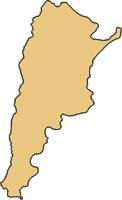
\includegraphics[width=0.6cm,height=1.2cm]{Imagenes/argentina.jpg}\\
\hline
2 & Brasil & 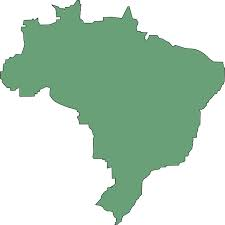
\includegraphics[width=1.5cm,height=1.5cm]{Imagenes/brasil.jpg}\\
\hline
\end{tabular}\\
\end{center}
\ \\
Y adem\'as brindar herramientas que permitan comparar eficientemente datos como los de la tercer columna.

\subsection*{Bases de Datos Espaciales}
\textbf{Definici\'on 1:} Es una Base de Datos que es optimizada para almacenar y consultar informaci\'on relacionada a objetos en el espacio, incluyendo puntos, l\'ineas y pol\'igonos.\\
\textbf{Definici\'on 2:} Es una colecci\'on de datos espaciales y no espaciales que est\'an interrelacionados.\\


\mychapter{5}{Bases de Datos Espacio-Temporales}

\bibliography{ref.bib}
\end{document}